\chapter{Design \& Implementation}
\label{ch:design-implementation}

\section{Language \& Machine Learning Framework}

% \begin{itemize}
%     \item Python as pre-existing machine learning frameworks
%     \item Tensorflow vs PyTorch (Tensorflow seemed nicer and more base code, first code seen for proof of concept was in tensorflow)
%     \item mutually exclusive due to CUDA implementations
% \end{itemize}

\subsection{Python}

When choosing a language to code this project in Python\footnote{\url{https://www.python.org}} was a clear choice. Whilst other languages offer better speed (C++\footnote{\url{https://cplusplus.com/}}, Rust\footnote{\url{https://www.rust-lang.org/}}), Python's advantage comes from its libraries.

Libraries are modular pieces of code written by other developers that can be integrated into a new software to make common tasks easier. In Python this is accomplished using the \verb|import| and \verb|from| syntax. Libraries vastly simplify coding as they can vastly reduce complex problems to simple functions. This is especially useful when dealing with complex machine learning functions, advanced mathematical algorithms such as Adam can be reduced to an import. Many Python libraries are written in lower-level languages like C or C++, allowing Python code to benefit from high performance while maintaining ease of use.

The vast majority of popular packages have a Python implementation that can be easily installed by the Python Package Index\footnote{\url{https://pypi.org/}}. Especially for machine learning, Python has some of the largest collection of relevant libraries of any language and is therefore the language of choice for this project.

\subsection{PyTorch versus TensorFlow}

There are many machine learning frameworks in Python, however the primary two are PyTorch\cite{paszke2019pytorch} and TensorFlow\cite{abadi2016tensorflow}. They both offer near identical feature sets and performance so choosing between them is not a simple matter.

PyTorch was created by Meta in 2019. It is a lot newer and viewed as a more ``pythonic" framework\cite{chirodea2021comparison}. To be more ``pythonic" is to be more developer-friendlier by providing a simple interface to the library that developers already familiar with Python should easily pick up on. PyTorch supports a dynamic computation graph which enables for dynamic changes of model architectures.

TensorFlow is a much more mature framework by Google releasing in 2015. It offers similar abstractions as PyTorch but is widely viewed to be slightly harder to develop in\cite{chirodea2021comparison}. TensorFlow uses an eager computation graph meaning no changes to model architectures can be made once a model is defined. Whilst this reduces flexibility during runtime, it allows for more optimisations to be made to the model architecture meaning greater accuracy, smaller model architectures, and sometimes quicker computations. TensorFlow also scales effectively running as efficiently as possible on desktop computers to large GPU clusters.

Unfortunately, TensorFlow and PyTorch are mutually exclusive. Both rely on separate versions of the CUDA backend to allow for GPU acceleration on NVIDIA architectures. Whilst this can be accomplished using virtually environments and other work arounds it is generally recommended to use one or the other.

Due to their similarities, there is no clear choice between PyTorch and TensorFlow. Some trends have emerged, however, with PyTorch being used for research and development work where iterative improvements are desired whereas as TensorFlow is employed for production environments. 

TensorFlow was chosen for this project for a number of reasons. Firstly, the flexibility that PyTorch offers is less important to this project as all models being used have had their architectures pre-defined. On the other hand, TensorFlow's ability to scale and optimise for the compute resources will be valuable for this project as it will be developed on smaller desktops but the final evaluation loops will be run on large GPU clusters. Furthermore, after trying out both TensorFlow and PyTorch, the author preferred the overall syntax of TensorFlow.

\section{Proof of Concept}
\label{sec:concept-design}

% \begin{itemize}
%     \item Re-use oriented design
%     \item Quick and dirty
%     \item test my theory
%     \item explain methodologies
% \end{itemize}

To validate whether blink-based DeepFake detection is resistant to adversarial noise, it was decided to construct a proof of concept during the Christmas holiday. As it is intended to be a small test-bed, small flaws in the design are acceptable. Therefore, it makes sense to use pre-existing models, solutions, and implementations where possible in order to speed up development.

The overall architecture of blink-based DeepFake detection is relatively simple. First, the landmarks around the face are computed to determine for every frame to generate an EAR-time graph. The graph can then be analysed to determine whether the video is real or not. 

\begin{algorithm}
    \caption{Overall architecture of a blink-based DeepFake detector}
    \label{alg:blink-based}
    \begin{algorithmic}
        \Require video
        \State ears $\gets$ \{\}
        \For{frame $\in$ video}
            \State landmarks $\gets$ \textsc{GetLandmarks}(frame)
            \State ear $\gets$ \textsc{CalculateEAR}(landmarks)
            \State \textsc{Append}(ears, ear)
        \EndFor
        \State classification $\gets$ \textsc{EARAnalysis}(ears)
    \end{algorithmic}
\end{algorithm}

It was decided to use an EAR-based approach over a custom blink model, because it allows for complex analysis. EAR data is more precise than the binary open/close of a custom model, allowing for analysis of not just frequency of blinks but more subtle details like how the blink starts and ends, the velocity of the eye, and whether the eye consistently returns to the same position when open. The flaws in EAR noted by Ictu Oculi\cite{li2018ictu} are valid but they rely on the eye landmarks being unreliably marked, with sufficiently advanced models trained with occlusions this can be overcome. 

To calculate the EAR, the six landmarks around the eye need to be located. Google's MediaPipe\cite{lugaresi2019mediapipe} was used for this purpose. It is designed to run in real-time on mobile devices and other edge compute resources and hence is very light weight and fast. MediaPipe produces 478 landmarks in three dimensions that cover the entire face, a subset of twelve (six landmarks per eye) is then used to be the six landmarks for EAR. From the six landmarks, the EAR can be calculated using Equation \ref{eq:ear} and the average taken for the final EAR-time graph. 

EAR analysis is performed using the hybrid of DeepVision\cite{jung2020deepvision} and Ictu Oculi\cite{li2018ictu} by counting the number of blinks in the EAR graph and comparing that to the human average. DeepVision's database was viewed as too time-consuming to produce and the simplicity of Ictu Oculi's approach was appealing for its speed advantage. In experiments, DeepVision's threshold of two standard deviations below the mean proved to be to inconsistent so a revised threshold of half a standard deviation above the minimum EAR value was chosen. The average human blinks 14 times per minute\cite{schiffman1990sensation}, DeepFakes will blink less than this and so if the subject of the video blinks less than 14 times a minute, the video is deemed as a fake.

For traditional detectors, both ResNet and VGG architectures have been proven vulnerable to adversarial noise\cite{gandhi2020adversarial}. A ResNet-based DeepFake detector was implemented using an implementation from Tiwari\cite{tiwari2024deepfake}, a VGG-detector was implemented using a header from Krishna et al\cite{krishna2022deepfake} but the backbone was upgraded to VGG19 following research from Yadav et al\cite{yadav2024deepfake}. To extend frame-by-frame detection to entire videos, each frame in a video is analysed independently. If the frame is classified as fake then a counter is incremented by one. If the counter exceeds a given threshold (set as one hundred frames), the video is classed as fake.

Adversarial noise was added to images using the Foolbox library\cite{rauber2017foolbox}\cite{rauber2017foolboxnative}. FGSM was used as the method for noise due to its known effectiveness and speed\cite{gandhi2020adversarial}. $\epsilon$ was set to 0.1. To replicate real life scenarios, noise was only added to faked videos and all models were solely trained on original videos, not noisy ones.

The models were trained on a subset of fifty real and fifty fake videos from the FaceForensics++ dataset\cite{roessler2018faceforensics}. Testing was run over a further fifty real and fifty fake videos. The results of the tests can be found in Section \ref{sec:concept-results}. FaceForensics++ was chosen as it was the most robust dataset available at the time. More have been tested in the main code. Hyperparameters for the VGG and ResNet models were left the same as the original implementations. To reduce overfitting, only one frame per second was extracted and used for training.

\section{Main DeepFake Detection Algorithm}

% \begin{itemize}
%     \item pseudocode of main algorithm
%     \item if at any point something fails, mark as fake (ensures resiliency)
%     \item emphasise each part is interchangeable
% \end{itemize}

The main DeepFake detection algorithm is similar to the one discussed in the proof of concept (Algorithm \ref{alg:blink-based}) in terms of structure. The code in the main algorithm is an alteration of the subroutine calls, making each subroutine return more accurate results. Other improvements were made such as general improving speed and modularity of the code. To further improve testing and evaluation, a number of different options for each component were developed as each section of the algorithm is interchangeable. 

To improve resiliency against adversarial noise attacks, the entire algorithm is fail negative. If any section of the algorithm were to fail then the video would be deemed a fake. For example, if no facial landmarks are detected in a frame, then the video is declared fake.

\subsection{Face cropping}
\label{sec:face-cropping}

One common feature across all DeepFake detection and facial landmarking models is that they perform best when the face being analyses fills the entire frame, because background information is irrelevant and can disrupt the model. As such, it is incredibly useful to have a preprocessing step which crops a frame to just the faces in the frame using a face detector model. 

One of the most efficient models available is YuNet\cite{wu2023yunet}. YuNet is designed to run in real time (approximately 1 millisecond per frame) on a CPU, whilst retaining a high degree of accuracy. It only contains 75,856 parameters, with many models requiring fifty times more parameters to reach similar levels of accuracy. More parameters means longer computation times, which was deemed unacceptable for a model designed to run on edge devices. With neural networks, quicker computation times often come at the expense of reduced accuracy; whilst this is still the case with YuNet, it still achieves ``similar accuracy to other small models" on standardised benchmarks. OpenCV contains an implementation of YuNet for use in Python\cite{yunetpyton}.

A more accurate CNN for detecting faces is Multitask Cascaded Convolutional Networks (MTCNN)\cite{zhang2016joint}. MTCNN is more accurate, achieving 0.851 mean average precision on benchmarks, compared to YuNet's 0.836. The accuracy comes with a significant speed decrease. Where YuNet takes one millisecond per frame, MTCNN takes ten milliseconds. The MTCNN library\cite{centeno2024mtcnn} is a popular Python implementation of MTCNN.

To attain the optimal combination of speed and accuracy both YuNet and MTCNN are used to identify faces in a video. An initial pass on all frames is done via YuNet, if no faces are found in a frame then MTCNN is used to identify the faces. To improve the performance of MTCNN, faces are processed in batches of 8. It was noted during testing that when exposed to adversarial noise, YuNet was prone to miss faces, as such the confidence YuNet required to mark a face was reduced from 0.9 to 0.7. Only the primary face in each frame is used, for the first frame this is taken as the face with highest confidence from the model, for subsequent frames it is the face with the smallest euclidean distance between the vertices of the bounding box. 

\begin{algorithm}
    \caption{The method for cropping faces from a video}
    \label{alg:face-detection}
    \begin{algorithmic}
        \Require video
        \State faces\_per\_frame $\gets$ \{\}
        \For{frame $\in$ video}
            \State faces\_coords $\gets$ \textsc{Yunet}(frame)
            \If{faces\_coords $\neq$ \{\}}
                \State \textsc{Append}(faces\_per\_frame, face\_coords)
            \Else
                \State faces\_coords $\gets$ \textsc{MTCNN}(frame)
                \State \textsc{Append}(faces\_per\_frame, face\_coords) \Comment{Will deliberately append empty set if no faces}
            \EndIf
        \EndFor
        \State faces $\gets$ \{\}
        \State previous\_face $\gets$ \{\}
        \For{frame\_faces$\in$ faces\_per\_frame}
            \State best\_face $\gets$ \{\}
            \If{previous\_face $=$ \{\}}
                \State best\_face $\gets$ frame\_faces[0]
            \Else
                \State best\_face $\gets$ \textsc{MinimumDistance}(frame\_faces,previous\_face)
            \EndIf
            \State previous\_face $\gets$ best\_face
            \State \textsc{Append}(faces, best\_face)
        \EndFor
    \end{algorithmic}
\end{algorithm}

\subsection{Eye Landmark Detection}

% \begin{itemize}
%     \item EAR needs 6 points per eye so lets get them
%     \item Facial landmarking is a common superset problem
%     \item Introduce 68 landmarks and datasets
%     \item Most popular ones aren't viable as built to be small to fit in a package (dlib, opencv...) or to run on a phone (mediapipe)
% \end{itemize}

To determine the EAR in a specific frame, the six landmarks around each eye need to be located. There are a large number of Python packages which come with facial landmarking features, unfortunately most of these are unsuitable for use in a state of the art detector as they are insufficiently accurate. The models included in packages are either compressed for ease of distribution or optimised to run on devices with reduced computational capabilities. 

\subsubsection{Weakly Supervised Eye Landmarks Detection}

% \begin{itemize}
%     \item Looked promising
%     \item Most accurate according to landmarks in paper \& only model focussing specifically on eye landmarking
%     \item Has a ``good enough" implementation details
%     \item Had issues
%     \begin{itemize}
%         \item Landmarks from regions (mention other paper that managed it
%         \item difficulty implementing in tensorflow
%         \item after a month scrapped development
%     \end{itemize}
% \end{itemize}

The first method researched for eye landmark detection was Weakly Supervised Eye Landmarks Detection (WSELD)\cite{huang2020eye}. In facial landmarking benchmarks (Section \ref{sec:face-datasets}), WSELD is the most accurate with respect to eye landmarking when compared to current state of the art methods on mean squared error loss.

A Regional-CNN (R-CNN)\cite{ren2015faster} outputs initial landmarks. R-CNNs are a special type of CNN that use Region of Interest (ROI) to locate objects within an input so that later layers can specifically focus on those regions. R-CNN consists of three primary components, a traditional CNN backbone for feature extraction, a Region Proposal Network (RPN) which selects hypothetical areas of interest, A final ROI pooling layer combines the features from the backbone with the regions to produce regions that can be used for future layers of the network. WSELD uses R-CNN to produce both eye bounding box regions (the regions of interest) and initial predictions of eye landmarks.

To augment the initial eye landmarks to final, precise landmarks, WSELD employs a custom RNN. The primary component of the RNN is an LSTM module which uses the previous predictions to refine the current prediction. Dense layers surround the LSTM unit to adapt the input and output data into usable formats.

An overall network diagram is shown in Figure \ref{fig:wseld}.

\begin{figure}[h]
    \centering
    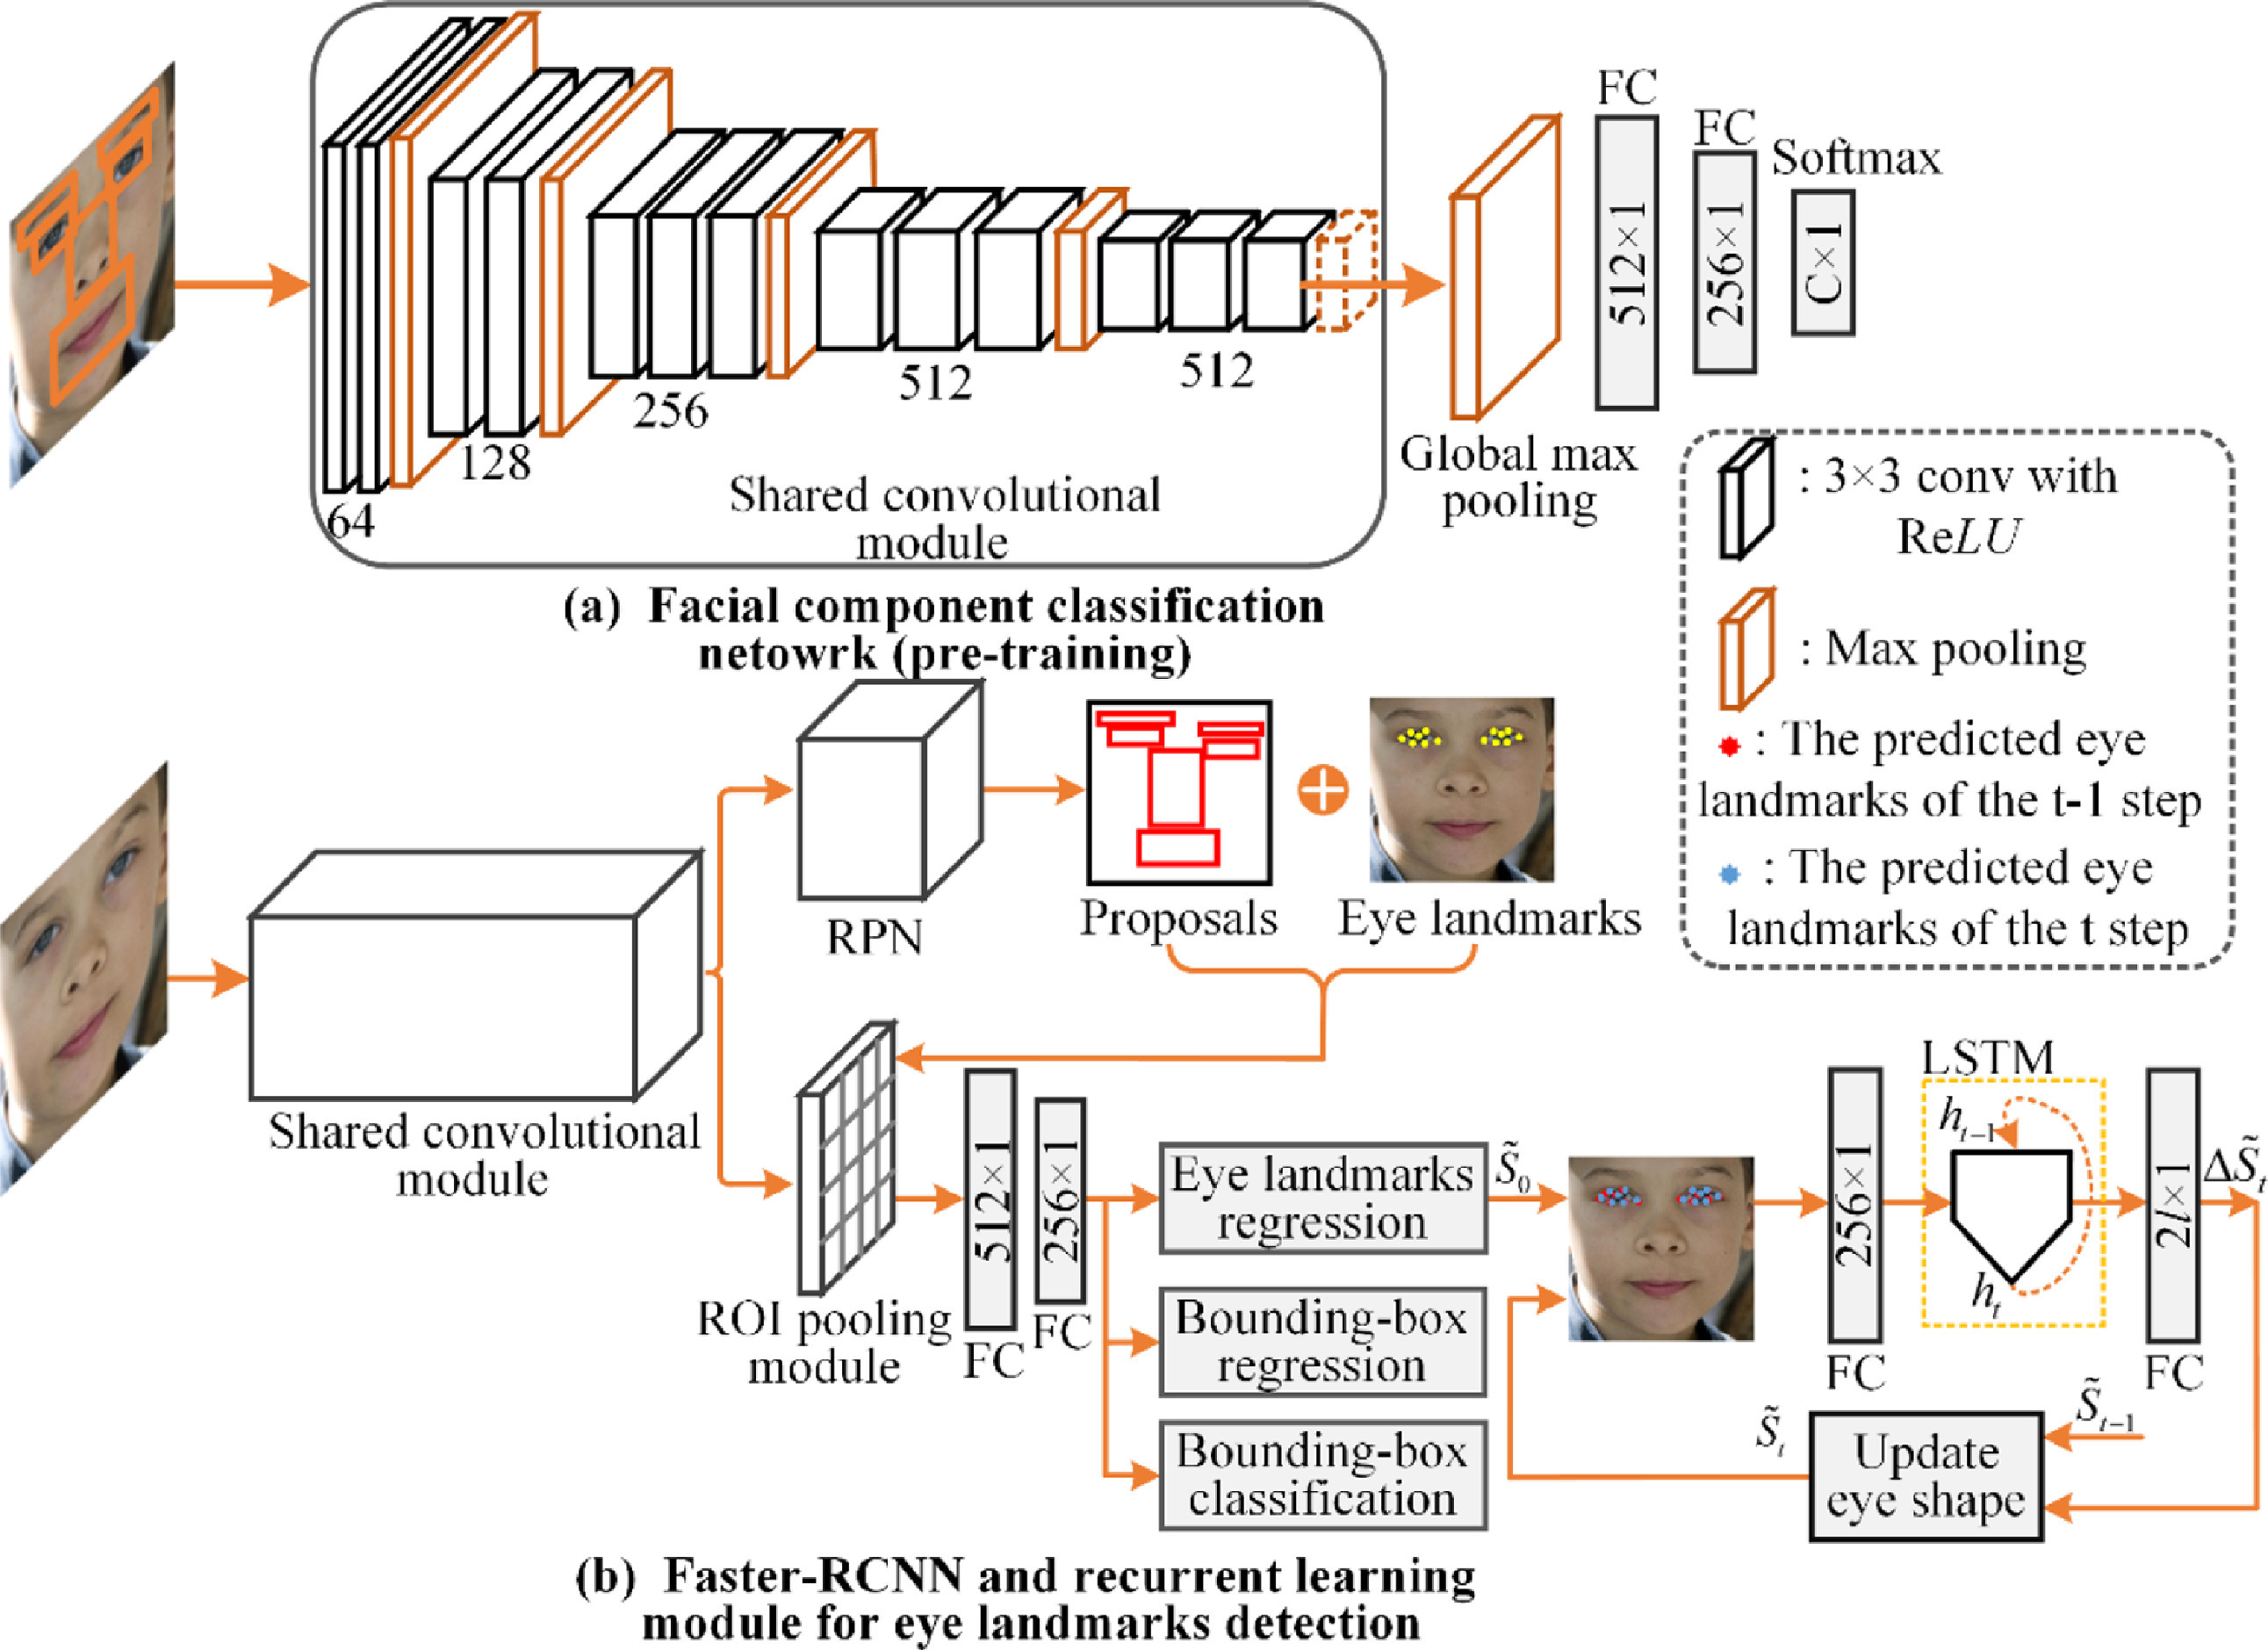
\includegraphics[width=0.75\linewidth]{dissertation//figures/wseld.jpg}
    \caption{Network diagram of Weakly Supervised Eye Landmarks Detection\cite{huang2020eye}}
    \label{fig:wseld}
\end{figure}

Whilst the original paper gave clear implementations, their code was difficult to replicate. No code was supplied with the paper so all code had to be generated from scratch. The most confusing aspect of the model was generating landmarks from an RPN. As the name suggests, RPNs are only able to generate regions, as such it would seem to be impossible to generate landmarks. A similar paper was able to produce results on multiple facial regions\cite{tang2018facial} but, again, no code was provided. In this implementation it was assumed a dense layer with the number of outputs equal to the number of landmarks was incorporated into the output of the RPN. Furthermore, this was the author's first time coding a substantial learning framework in TensorFlow. There is no pre-built RPN module so one needs to be created from scratch, a number of open source implementations exist\cite{hxuaj2021tensorflow2}\cite{kewar2021region} but these do not generate landmarks. It was attempted to create a custom R-CNN but there was a seeming constant stream of bugs. The bugs, along with there being no way to confirm whether the method of adding landmarks to RPN was successful resulted in development of WSELD being halted in favour of a new facial landmarking network.

\subsubsection{Pre-implemented Models}

% \begin{itemize}
%     \item Re-use oriented design
%     \item papers with code
%     \item Used best models which had pre-existing implementations (one for fast, one more accurate)
%     \item couldve optimised for 6 landmarks but didnt want to mess with model architectures that were known working (batch size probably meant nothing would change anyway)
% \end{itemize}

To avoid a repetition of the WSELD implementation, it was decided to switch to a re-use oriented methodology for facial landmarking. In order for a model to be considered, it must have an open source implementation available. PapersWithCode\footnote{\url{https://paperswithcode.com}} is an aggregation site which ranks models on popular machine learning problems and links to known codebases where possible. 

The facial landmark detection is a common problem in machine learning. The vast majority of available training datasets (Section \ref{sec:face-datasets}) contain the six points required for EAR calculation and as such any model that can be trained on these datasets can be used for eye landmarking. In theory, it is possible to optimise the networks for solely eye landmark detection, however this will not be optimised due to the potential that had to disrupt a network that is known to be working.

\subsubsection{High-Resolution Network}

% \begin{itemize}
%     \item modular sequences
%     \item keeps high resolution layers in context at all times
%     \item generic network but with a specific implementation for eye landmarking
%     \item Heatmap per landmark
% \end{itemize}

The most implemented facial landmark detector on PapersWithCode is High-Resolution Network (HRNet)\cite{sun2019high}. HRNet is actually a proposal for a novel architecture of CNNs that has applications in many fields and one of those fields is facial landmarking.

HRNet's novel contribution is CNNs working in parallel. Typical CNNs have one layer following another, whilst HRNet contains multiple CNNs in parallel, each working at a different resolution over the image. Similar to a CNN, the network gradually introduces lower and lower resolution layers to focus on more generic features, but at all times keeps the higher resolution layers in context which can refine their feature predictions based on the input from more lower level feature predictions. Lower resolution layers are connected to higher resolution layers through fusion layers which either upsample or downsample the feature predictions using either a CNN for downsampling or a bilinear for upsampling. An overview of the architecture for a HRNet is shown in Figure \ref{fig:hrnet-diagram}.

\begin{figure}[h]
    \centering
    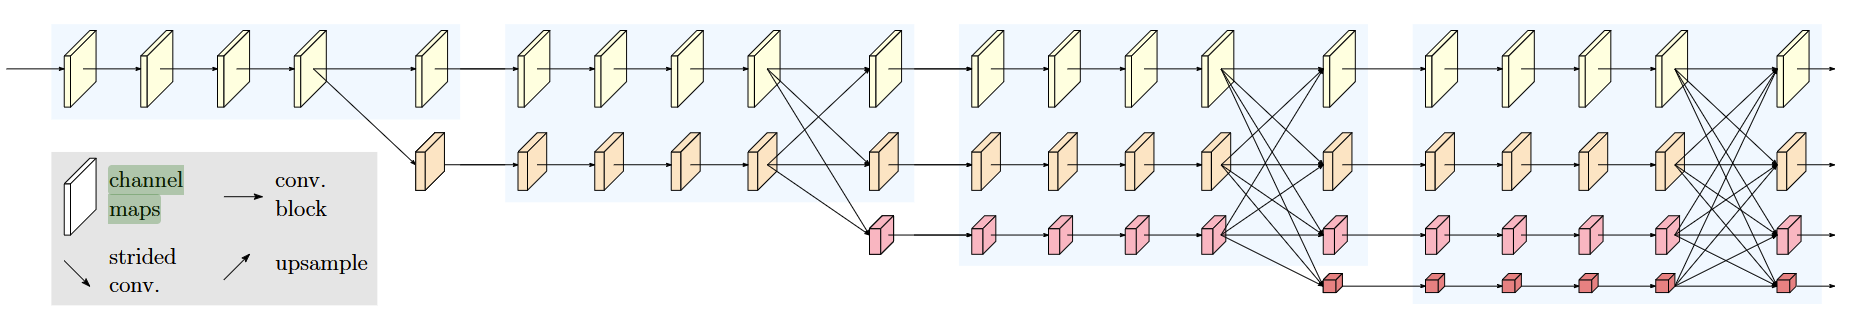
\includegraphics[width=1\linewidth]{dissertation//figures/hrnet-network.png}
    \caption{A generic network diagram for a High-Resolution Network\cite{sun2019high}}
    \label{fig:hrnet-diagram}
\end{figure}

Whilst HRNet is a generic architecture, it has been applied with great effect to facial landmarking. Such an implementation has been made open source in HRNet's official GitHub repository\cite{zhao2019facial} which details the specific architecture used of HRNet uses for facial landmarking. Similar to Figure \ref{fig:hrnet-diagram}, the network consists of four distinct modules, with each module containing four convolutional layers. Each module introduces one additional parallel network. Each layer consists of 18, 36, 72, and 144 filters respectively.

Instead of a set of coordinates for landmarks, the output of HRNet is a heatmap of the likely locations of a landmark with the peak of the heatmap being the most probable location (Figure \ref{fig:hrnet-output}. As such the location of the maximal value of the heatmap can be taken as the final location of a landmark. Whilst a simple version would be to simply take the index of the maximal value in the array, this neglects the possibility of the landmark being in the subpixel domain. The output heatmap is relatively low resolution ($64\times64$) and so it is highly likely the peak is within a subpixel. The problem has been research by Fisher et al.\cite{fisher1996comparison}. The most accurate algorithm proposed is Centre of Mass 7 (CoM7) which assumes the heatmap follows a Gaussian distribution and can therefore be estimated using a weighted average as shown through Equation \ref{eq:com7}. Firstly, the coordinates of the maximal value are computed and stored as $x,y$. Six values on either side of the maximal value are retrieved ($f(x)$). The original equation assumes one dimension, but it can be expanded to two by performing the calculation twice, one for $x$ and one for $y$.

\begin{figure}[h]
    \centering
    \begin{subfigure}{0.25\textwidth}
        \centering
        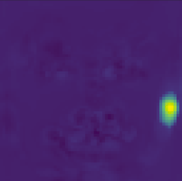
\includegraphics[width=\textwidth]{dissertation/figures/hrnet-single.png}
        \caption{The heatmap for a single landmark}
        \label{fig:hrnet-single}
    \end{subfigure}
    \hspace{3cm}
    \begin{subfigure}{0.25\textwidth}
        \centering
        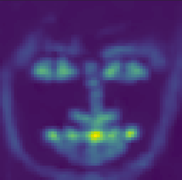
\includegraphics[width=\textwidth]{dissertation/figures/hrnet-multiple.png}
        \caption{The heatmap for all facial landmarks}
        \label{fig:hrnet-multiple}
    \end{subfigure}
    \caption{The heatmap outputs of HRNet}
    \label{fig:hrnet-output}
\end{figure}

\begin{equation}
    \label{eq:com7}
    \hat{x} = \frac{3f(x+3)+2f(x+2)+f(x+1)-f(x-1)-2f(x-2)-3f(x-3)}{f(x+3)+f(x+2)+f(x+1)+f(x)+f(x-1)+f(x-2)+f(x-3)}
\end{equation}

HRNet achieves state of the art performance on facial landmarking datasets. It is currently ranked in the top 25 on a variety of datasets by the PapersWithCode\cite{paperswithcodehrnet}. As there are multiple CNNs working in parallel, HRNet is often slower than a CNN on equivalent tasks. When trained, HRNet operates at approximately 30 frames per second when run on an RTX3060ti. As such, HRNet is not viable for real time computation on edge devices but can be used for detection on powerful machines.

When training, the ground truth heatmap was generated by centring Gaussian noise with a $\sigma=1.5$ on the true landmark, all other values in the heatmap were set to 0. Following the HRNet code\cite{zhao2019facial}, each heatmap was $64\times64$. To align with the inputs for all the other models used in this project, the input was scaled up from $112\times112$ to $256\times256$. The model was trained for 60 epochs with mean squared error as the loss and the Adam\cite{kingma2014adam} optimiser.


\subsubsection{Practical Facial Landmark Detector}

% \begin{itemize}
%     \item speedy boi
%     \item uses mobilenet-techniques to reduce the size and increase the speed
%     \item still accurate tho
%     \item secret sauce is custom loss function
% \end{itemize}

A Practical Facial Landmark Detector (PFLD)\cite{guo2019pfld} is an accurate landmarker that is primarily designed for speed. Developed to run on edge devices such as phones, the model can achieve speeds of 150 frames per second on some phones with a minimal reduction in accuracy.

The architecture of PFLD is more a similar to a traditional CNN: a backbone that leads into a number of dense layers which produce the final classification. PFLD uses the MobileNet backbone\cite{howard2017mobilenets} for feature extraction. MobileNet is a lightweight neural network specifically designed to be as small and as fast as possible, similar to the ideals of PFLD. 

MobileNet is built upon depthwise separable convolutions. A traditional convolutional layer will analyse every channel of an input (such as the red, green, and blue channels in an image) at once, combining them in a single step, for every pixel in an image. A depthwise separable convolution layer instead analyses each input channel independently, and then combines them afterwards. This vastly reduces the computation required as learnable parameters are separated from each other in different stages, as such when combined over larger images the parameters combine linearly rather than exponentially, reducing computation costs. 

Bottlenecks further speed-up MobileNet by reducing the dimensions of feature vectors. As data flows through a traditional CNN it can reach into a large number of dimensions, bottlenecks reduce the dimensions of a neural network which exponentially increase the network's speed. Bottlenecks reduce the dimension by having fewer neurons than the layer before it, forcing data to be aggregated and hence reducing complexity.

MobileNet also comes with a width hyperparameter that can further narrow down a network, increasing speed at the expense of accuracy. For this project, accuracy is more important than speed so only the most accurate MobileNet model is used, as such the width parameter is set to $1\times$. 

PFLD also includes an auxiliary network that is only used for training. To improve accuracy in a small network, PFLD uses a custom loss function which requires the pitch, yaw, and roll of a face. Whilst these could be calculated from the landmarks produced by the PFLD network, during the early stages, this is very inaccurate and can cause the model learning to stall. The auxiliary network picks up from an intermediary layer midway through the main backbone and outputs three values which are the pitch, yaw, roll.

The overall main backbone is taken from the a PyTorch implementation\cite{zhao2019pfld} but with header from a TensorFlow fork\cite{qi2019pfld} to align with the number of facial landmarks required.
 
{\huge need to add own PFLD network diagram}

One of the key contributions to PFLD's accuracy is a custom loss function. A typical facial landmarking model will use some form of distance metric for the loss function. These can only be done in two dimensions, neglecting geometric and structural information. For example, the more you turn your head with respect to a camera, the closer your eyes will appear to the camera despite them remaining the same distant apart in three dimensional space. Whilst large scale models can get away with using conventional loss functions and brute force their way the inconsistencies, smaller models cannot. To take into account geometrical information, PFLD uses the pitch, yaw, and roll of a face from the auxiliary network to compute the following loss function:

\begin{equation}
    L =\sum^N_{n=1}\left(\sum^C_{c=1}\omega^c_n\sum^K_{k=1}(1-\cos{\theta^k_n})\right) ||d_n||^2_2
\end{equation}

$n$ represents the $n^\text{th}$ of $N$ landmarks. $C$ and $\omega$ are weighting parameters to equalise datasets. The dataset is divided into $C$ classes. A number of classes are proposed, but these require augmenting the dataset with hand labelled, as this is an individual project and some facial landmark datasets contain over 10,000 images (Section \ref{sec:face-datasets}) these weights are omitted. The primary weighting parameter is $\theta^1, \theta^2,\theta^3$ which represent the difference the difference between the estimated and truth pitch, yaw, and roll respectively. As the delta goes up, so does the penalisation allowing the model to compensate for large deviations in head poses. Finally, L2 loss ($||d_n||^2_2$) is used as the primary loss component that is then weighted by the previous factors. 

To find the ground truth angles of the face, the Perspective-n-Point algorithm\cite{mallick2016head}\cite{hou2018face} maps sample points in three dimensions to two dimensions on the face, from which the facial angles can be calculated. The model was trained for 500 epochs following the PyTorch implementation\cite{zhang2016joint} using the Adam\cite{kingma2014adam} optimiser.

\subsubsection{Facial Landmark Datasets}
\label{sec:face-datasets}

% \begin{itemize}
%     \item 68 landmarks (upsampling and downsampling where necessary)
%     \item list all of them and give brief overview
%     \item didnt use aflw due to inaccurate landmarks or not enough landmarks
%     \item reflected to double size
% \end{itemize}

Similar to DeepFake detection (Section \ref{sec:datasets}), large numbers of faces have been pulled from the internet and hand labelled to enable the training and comparison of accurate facial landmarking models. The precise number of landmarks varies but the standard is 68 with some datasets labelling more landmarks, acting as a superset. 68 landmarks was used for this project as only the six eye landmarks for calculating the EAR are useful and the 68 landmarks is the smallest standardised size that covers all of them. Reducing the number of outputs significantly speeds up the model as less nodes are required to be trained. Where a model used more than 68 landmarks, a mapping was made from the model's landmarks to the main 68 and the rest of the landmarks were discarded.

\begin{figure}[h]
    \centering
    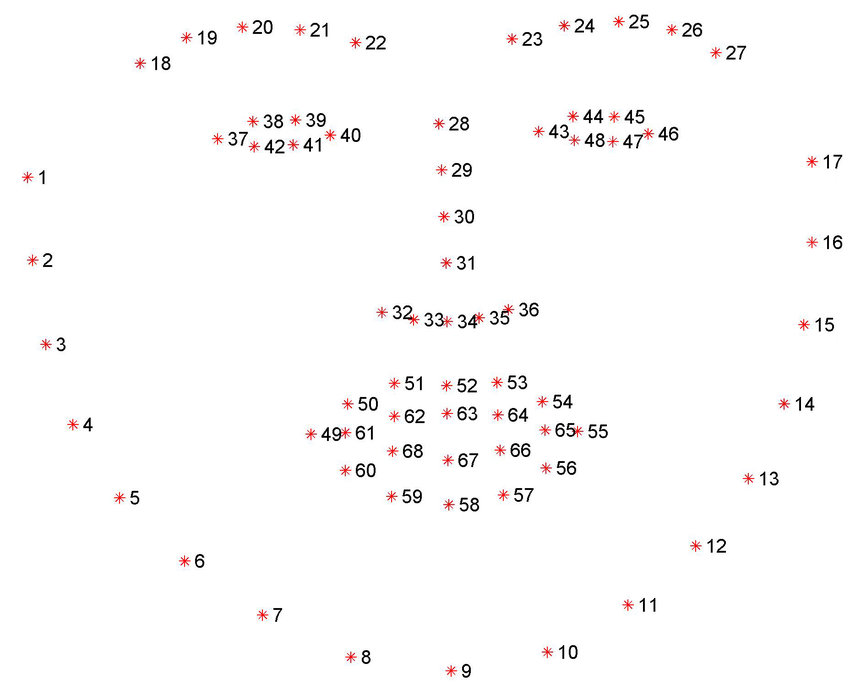
\includegraphics[width=0.5\linewidth]{dissertation//figures/facial-landmarks.jpg}
    \caption{68 facial landmarks}
    \label{fig:facial-landarks}
\end{figure}

A variety of datasets were chosen with the primary aim to include a wide variety of facial poses, environmental factors, and occlusions. Increasing the variety of data allows for the model to learn in more challenging scenarios and hopefully become more robust.

The following datasets were used: 300W\cite{sagonas2016300}\cite{sagonas2013300}\cite{sagonas2013semi}, Labelled Face Parts in the Wild (LFPW)\cite{belhumeur2013localizing}\cite{mondal2021lfpw}, Caltech Occluded Faces in the Wild (COFW)\cite{burgos2022caltech}, Annotated Faces in the Wild\cite{zhu2012face}, HELEN\cite{le2012interactive}, and Wider Facial Landmarks in the Wild (WFLW)\cite{wayne2018lab}.

In total these contain 11,495 labelled images. A common method of augmenting the dataset is to flip the images horizontally, which increases the dataset to 22,990 image. Data is scraped from a variety of imaging sites such as Flickr\footnote{\url{https://www.flickr.com/}}, Google\footnote{\url{https://images.google.co.uk/}}, and Yahoo!\footnote{\url{https://images.search.yahoo.com/}}. The dataset is very comprehensive covering a wide variety of individual characteristics like age, gender, and race. Environmental factors are also covered such as lighting, whether the photo was taken outside or inside. 
Two datasets (COFW and WFLW) were specifically chosen for their coverage of facial occlusions. Occlusions are where certain landmarks are obstructed from the view of the camera, for example sun glasses blocking eyes and hair obscuring one side of the face. Some examples of occlusions are shown in Figure \ref{fig:occlusions}.

\begin{figure}[h]
    \centering
    \begin{subfigure}{0.45\textwidth}
        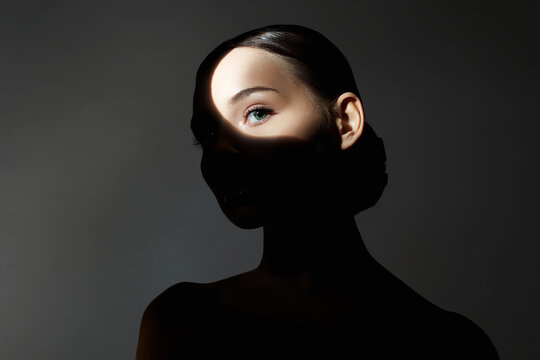
\includegraphics[width=1\linewidth]{dissertation//figures/shadow.jpg}
        \caption{A face occluded by shadow}
        \label{fig:occlusion-shadow}
    \end{subfigure}
    \hfill
    \begin{subfigure}{0.45\textwidth}
        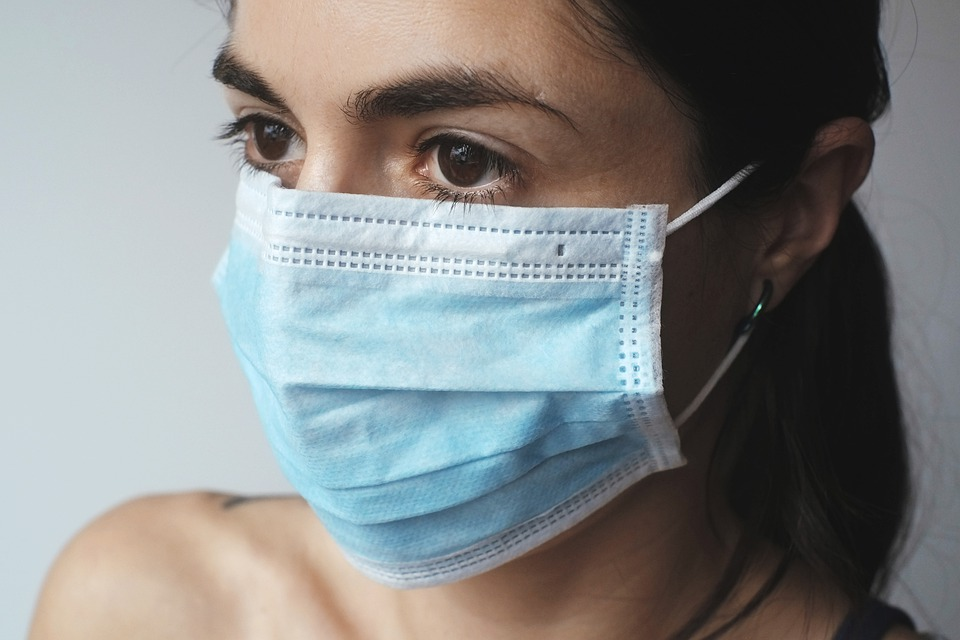
\includegraphics[width=1\linewidth]{dissertation//figures/occlusion-mask.jpg}
        \caption{A face occluded by a mask}
        \label{fig:occlusion:mask}
    \end{subfigure}
    \caption{Faces that have been partially occluded}
    \label{fig:occlusions}
\end{figure}

As explained in Section \ref{sec:face-cropping}, landmarking models benefit from faces filling the majority of images. To account for this, when training, the images are cropped to the facial region. This region is defined as the area bounded by the ground truth eye landmarks with 2\% padding on each side.

\subsection{Eye Aspect Ratio Analysis}

% \begin{itemize}
%     \item Can be abstracted to a univariate time series
%     \item Well researched
%     \item Classical methods exists (pyts library)
%     \item explain each one and give simple summary (1 paragraph)
%     \item As do deep learning frameworks (the other papers)
%     \item model diagrams for each one (maybe give a rough explanation as to the aims each one is doing?)
% \end{itemize}

With the eye landmarks located and the EAR calculated for each frame, the result is an EAR-time graph (Figure \ref{fig:real-ear-graph}). Existing blink-based DeepFake detectors will extract features from the graph such as frequency and period. A novel approach from this project is to use the entire EAR graph for analysis by abstracting the problem into univariate time series classification.

\begin{figure}[h]
    \centering
    \includegraphics[width=0.5\linewidth]{dissertation/figures/real-ear-graph.png}
    \caption{A sample graph of EAR over frame of video}
    \label{fig:real-ear-graph}
\end{figure}

A univariate time series is a single point of data that varies over time. A large amount of research has been dome into time series due to their frequent appearance in statistical models. Traditionally machine learning models struggle with temporal structures seen in time series but over time reliable methods have been developed. A comprehensive overview of state of the art time series algorithms for time series classification has been provided Johann Faouzi\cite{faouzi2024time}.

\subsubsection{K-Nearest Neighbours with Dynamic Time Warping}

K-Nearest Neighbours (k-NN) is a common algorithm for classification problems. Points are plotted in $n$ dimensional space

\subsubsection{Learning Shapelets}

\subsubsection{Time Series Forest}

\subsubsection{Time Series Bag-of-Features}

\subsubsection{Neural Networks}

\subsubsection{Implementation}

\section{Adversarial Noise}

\begin{itemize}
    \item foolbox library (Targeted FGSM using the other thing)
    \item chosen over cleverhans as cleverhans had meh documentation
    \item cw-l2 attack too slow (3hrs per video)
    \item fakeretouch has no open-source implementation, timings were too slow, estimated would also take a while
\end{itemize}

\section{Final Code}

\begin{itemize}
    \item One codebase to do full training, splitting and evaluation
    \item just give overall flow diagram?
    \item {\huge models only trained on non-noisy images}
    \item checkpointing where possible
    \item run on either dcs compute clusters or avon
    \item final speeds + hardware
\end{itemize}